\documentclass{article}
\usepackage{protools}
\setlength\parskip{0.25\baselineskip}

\addbibresource{towards.bib}

\begin{document}

\ArticleTitle
  {Towards Optical States Of Four Photons}
\ArticleAuthor*
  [0000-0002-5646-6964]
  {Jan Provazn\'{i}k}
  {provaznik@optics.upol.cz}
\ArticleAuthorAddress
  {Department of Optics, Palack\'{y} University, 17. listopadu 1192/12, 771 46 Olomouc, Czech Republic}

\ArticleAuthor
  {Olga Solodovnikova}
\ArticleAuthorAddress
  {Technical University of Denmark, Lyngby, Denmark}

\ArticleAuthor
  [0000-0002-5761-8966]
  {Petr Marek}
\ArticleAuthorAddress
  {Department of Optics, Palack\'{y} University, 17. listopadu 1192/12, 771 46 Olomouc, Czech Republic}

\ArticleAuthor
  [0000-0003-4114-6068]
  {Radim Filip}
\ArticleAuthorAddress
  {Department of Optics, Palack\'{y} University, 17. listopadu 1192/12, 771 46 Olomouc, Czech Republic}

\ArticleTitlePrint

\begin{abstract}\noindent
  Quantum non-Gaussian states and operations are a crucial component of quantum information processing protocols, but alas, both the realization of non-Gaussian operations for travelling modes of light and the preparation of non-Gaussian states pose significant practical challenges in contemporary experiments. In this paper, we discuss the minimal requirements imposed on the quantum efficiency of photon number resolving detectors and the quality of the squeezing operation in experimental realization of certifiable quantum non-Gaussian states of individual photonic states with three, four, and five photons.
\end{abstract}

% Introduction
%
%

\section{Introduction}

A measurement-based method for preparation of individual photonic states of light~\cite{yukawa2013a,yoshikawa2018,tiedau2019,provaznik2020} is discussed in the first section of this chapter. The mathematical model of the procedure takes loss into account, both in the construction of the state in during its characterization. The resulting states are certified using hierarchical criteria~\cite{lachman2019} in the second section by evaluating the statistical behavior of the model under realistic experimental conditions. Figures presented in this section can be used to determine the minimal requirements on the efficiency of the optical components, such as squeezing and detection, in experimental realizations targeting states of two, three, and four photons.

% Methodology
%
%

\begin{figure}[h]
  \begin{center}
    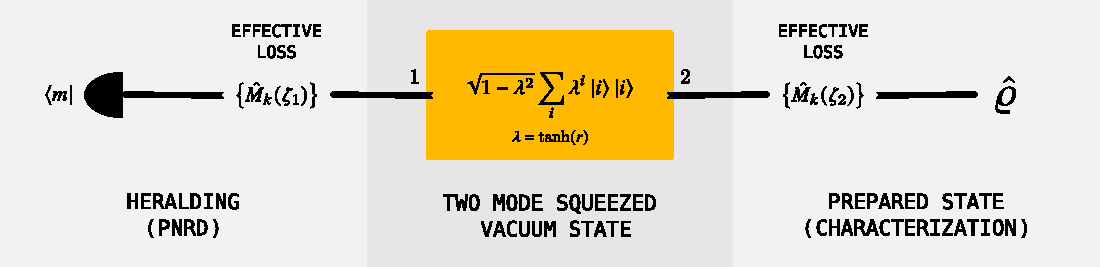
\includegraphics[width = 1.00 \columnwidth]{import/illustrate_scheme_alt.pdf}
  \end{center}
  \caption{
    Schematic illustration of the non-Gaussian state preparation circuit with a two mode squeezed vacuum state serving as a source of entangled quantum states. One of the modes is measured, thus projecting the other mode onto the resolved Fock state. 
  }
  \label{f-scheme}
\end{figure}


\section{Cooking up states of travelling light}

Photonic Fock states can be conditionally prepared by using a two mode squeezed vacuum state and a photon number resolving detector~\cite{yukawa2013a,yoshikawa2018,tiedau2019,provaznik2020}. The theoretical model of the experimental scheme is illustrated in~\figref{f-scheme}. One of the entangled modes is measured, thus projecting the other mode onto the resolved Fock state. This procedure is repeated until a satisfactory detection outcome in the heralding mode is observed, at which point the target state is successfully prepared. In the case of unfavourable detection event, the state is discarded and the whole procedure repeated.

One of the major experimental challenges in preparation of quantum states of light is the omnipresent loss and noise. It diminishes quantum correlations between entangled resources and reduces the quantum efficiency of detectors, making it impossible to prepare the desired quantum state with perfect fidelity. The reduced detection efficiency negatively affects both the preparation of the quantum state and its subsequent characterization. The procedure outlined in \figref{f-scheme} assumes a perfectly squeezed state and an ideal photon number resolving (PNR) detector. The adverse effects of realistic inefficiencies can be effectively accounted for by considering lossy transmission of both modes prior to their measurement with ideal detectors~\cite{feito2009}. 

The resulting non-normalized marginal state is given by
%
\begin{equation}\label{e-pnr-rho}
  \hatrho_{(m)} \approx
  \sum_{i = 0}^{\infty} 
  \sum_{j = 0}^{\infty}
    \lambda^{i} \lambda^{j}
    \left(
      \sum_{k = 0}^{\infty}
        \bra{m} \hat{M}_{k} (\zeta_{1}) \ketbra{i}{j} \hat{M}_{k}^{\dagger} (\zeta_{1}) \ket{m}
    \right)
    \left(
      \sum_{k = 0}^{\infty}
        \hat{M}_{k}(\zeta_{2}) \ketbra{i}{j} \hat{M}_{k}^{\dagger} (\zeta_{2})
    \right) \Qc
\end{equation}
%
where~$m$ identifies the detected Fock state,~${\lambda = \tanh(r)}$ characterizes the two mode squeezed state with initial squeezing~$r$, and the Kraus operators~${\hat{M}_{k} (\zeta)}$ describe the transmission loss with
%
\begin{equation}
  \hat{M}_{k} (\zeta) =
    \sqrt{ \frac{(1 - \zeta)^{k}}{k!} } 
    \sqrt{\zeta}^{\hat{n}} \hat{a}^{k}
\end{equation}
%
where~$\zeta$ gives the intensity transmittance of the lossy channel~\cite{ivan2011}. In the case of~\eqref{e-pnr-rho}, the parameter~$\zeta_{1}$ corresponds to loss in the first mode, called the heralding mode, whereas~$\zeta_{2}$ describes the loss affecting the mode carrying the prepared state.

The probability of successful preparation, that is, the probability of detecting~$m$ photons in the heralding mode, can be obtained analytically as
%
\begin{equation}\label{e-pnr-pro}
  P_{(m)} = (1 - \lambda^{2}) 
  \frac
    { (\lambda^{2} \zeta_{1})^{m} }
    { [ 1 - \lambda^{2} (1 - \zeta_{1}) ]^{m + 1} } \Qd
\end{equation}
%
The equation~\eqref{e-pnr-rho} for the resulting density matrix of the prepared state can be simplified. The matrix is diagonal in the Fock basis; its properly normalized elements are obtained as
%
\begin{equation}\label{e-pnr-rho-kk}
  \braket{ k | \hatrho_{(m)} | k } =
  \frac
    { [ 1 - \lambda^{2} (1 - \zeta_{1}) ]^{m + 1} }
    { [ \lambda^{2} (1 - \zeta_{1}) ]^{m} }
  \left( \frac{ \zeta_{2} }{ 1 - \zeta_{2} } \right)^{k}
  H (k, m, x) \Qc
\end{equation}
%
where the substitution~${x \coloneqq \lambda^{2} ( 1 - \zeta_{1} )(1 - \zeta_{2} )}$ is used in the function~$H(k, m, x)$ defined as
%
\begin{equation}\label{e-H}
  H(k, m, x) \coloneq
  \begin{dcases}
    \sum_{l = m}^{\infty}
      \binom{l}{m}
      \binom{l}{k}
      x^{l} 
    & k \leq m \Qc \\
    \sum_{l = k}^{\infty}
      \binom{l}{m}
      \binom{l}{k}
      x^{l}
    & k > m \Qd
  \end{dcases}
\end{equation}
%
The series in~\eqref{e-H} converge since~${\lambda^{2} ( 1 - \zeta_{1} )(1 - \zeta_{2} ) \leq 1}$. The infinite series in the formula can be alternatively expressed in terms of hypergeometric functions~\cite{bateman1981}, leading to the expression
%
\begin{equation}
  H(k, m, x) \equiv
  \begin{dcases}
    x^{m} \binom{m}{k} {}_{2}F_{1} (1 + m, 1 + m, 1 + m - k, x)
    & k \leq m \Qc \\
    x^{k} \binom{k}{m} {}_{2}F_{1} (1 + k, 1 + k, 1 + k - m, x)
    & k > m \Qc
  \end{dcases}
\end{equation}
%
which can be evaluated with the help of commonly available numerical libraries~\cite{virtanen2020}.

\subsection*{Approximate photon number resolving detectors}
% with capacity to approximate actual PNR detectors, 

The model of state preparation, represented by relation~\eqref{e-pnr-rho}, relies on true PNR detectors in the heralding stage of the circuit. While these detectors exist in principle~\cite{hopker2019,endo2021,endo2024}, their practical availability is severely limited. The model of the experimental circuit can be extended to cover the more commonly available cascaded avalanche photodiode~(CAP) detectors~\cite{hlousek2019,grygar2022,hlousek2024,ercolano2024} that operate by dividing the incoming signal equally between~$n$ independent avalanche photodiode detectors and counting the number~$m$ of detectors that registered photons. 
The avalanche detectors can only distinguish between zero and non-zero numbers of incident photons. This hinders the possibility of photon number resolution by the cascade. It approximates true PNR detectors well only in the limit of large numbers~$n$ of the constituent avalanche detectors~\cite{provaznik2020}. The detection events when~$m$ out of the~$n$ detectors register photons are associated with the positive operators~\cite{paul1996}
%
\begin{equation}\label{e-cap}
  \begin{gathered}
  \hat{\Pi}_{m}^{n} 
    \coloneqq \sum_{i = 0}^{\infty} w(i, m, n) \ketbra{i}{i} \\
  \text{where} \quad
  w(i, m, n) 
    \coloneqq 
    \begin{dcases}
      \; \frac{1}{n^{i}} \binom{n}{m} \sum_{j = 0}^{m} \binom{m}{j} (-1)^{j} (m - j)^{i} 
      & \text{when}\quad i \geq m \\
      \; 0 & \text{otherwise} \Qd
    \end{dcases}
  \end{gathered}
\end{equation} 
%
The relations~\eqref{e-pnr-pro} and~\eqref{e-pnr-rho} can be readily adapted to the use of CAP detectors. The resulting probability of success, obtained when heralding on the~$\hat{\Pi}_{m}^{n}$ outcome, 
%
\begin{equation}\label{e-cap-pro}
  P_{(m, n)} = \sum_{i = 0}^{\infty} w(i, m, n) P_{(i)} \Qc
\end{equation}
%
is the weighted average of the individual probabilities. The operator~\eqref{e-cap} of the measurement outcome and the original density matrix~\eqref{e-pnr-rho-kk} are diagonal in Fock representation; the resulting density matrix also retains its diagonal structure. Its respective elements 
are determined as a weighted average,
%
\begin{equation}\label{e-cap-rho-kk}
  \braket{k|\hatrho_{(m, n)}|k} =
    \frac{1}{ P_{(m,n)} }
    { \sum_{i = 0}^{\infty} w(i, m, n) P_{(i)} \braket{k|\hatrho_{(i)}|k} }
  \Qd
\end{equation}

% \begin{equation}\label{e-cap-rho}
%   \hatrho_{(m, n)} =
%     \frac{1}{ P_{(m,n)} }
%     { \sum_{i = 0}^{\infty} w(i, m, n) P_{(i)} \hatrho_{(i)} }
%   \Qd
% \end{equation}
% %
% Both the measurement outcome operator~\eqref{e-cap} and the original density matrix~\eqref{e-pnr-rho-kk} are diagonal in Fock representation. The resulting density matrix also retains its diagonal structure,
% %
%

% Certification
%
%

\subsection*{Genuine quantum non-Gaussian states}

Realistic inefficiencies in all the stages of the state preparation procedure are modeled with lossy channels. The reduced heralding efficiency makes it impossible to create the desired state with perfect fidelity. Effects of loss incurred during its characterization further diminish the already imperfect state. This can be partly alleviated using special hierarchical criteria~\cite{lachman2019}, closely related to the stellar rank~\cite{chabaud2020,walschaers2021,fiurasek2022} of the prepared state, as their invariance under Gaussian operations offers a certain degree of robustness against loss~\cite{lachman2019}.

Quantum states which can not be decomposed into statistical mixtures of pure states attainable by Gaussian transformations of superposed Fock states up to ${\ket{m - 1}}$ are called genuine $m$-photon quantum non-Gaussian ($m$-PQnG) states~\cite{lachman2019}. 
%
A quantum state~$\hatrho$ belongs to a particular $m$-PQnG hierarchy when the probabilities of its first $m$ photonic contributions
satisfy the inequality~${y_{m} \geq F_{m} (x_{m})}$ with the variables determined by
%
\begin{equation}
  x_{m} 
    = \sum_{k = m + 1}^{\infty} 
      \braket{k | \hatrho | k}
    = 1 - \sum_{k = 0}^{m} 
      \braket{k | \hatrho | k}
  \quad\text{and}\quad
  y_{m} = \braket{m | \hatrho | m}
  \Qc
\end{equation}
%
and the threshold function $F_{m}(x)$ obtained through sophisticated numerical optimization~\cite{lachman2019,fiurasek2022}.

% Monte Carlo Simulation
%
%

\subsection*{Monte Carlo simulation of the state preparation circuit}

The maximal tolerable amount of loss present in the optical circuit capable of preparing a certifiable genuine $m$-PQnG state can be determined by numerically simulating the experiment. The measurement statistics of a realistic experiment can be emulated using a Monte Carlo simulation based on the theoretical model of the circuit. Depending on the choice of heralding detectors used in the experiment, the relations~\eqref{e-pnr-rho-kk}~and~\eqref{e-cap-rho-kk} determine the diagonal elements of the conditionally prepared quantum state. Both relations are functions of the initial squeezing rate~$r$, the transmittances~$\zeta_{1}$ and~$\zeta_{2}$ of the lossy channels hindering both modes, and the post-selection criteria imposed on the measurement outcome $m$. The choice of the heralding detectors does not affect the methodology of the simulation and the subsequent state certification. The following description is therefore given in terms of the simpler relation~\eqref{e-pnr-rho-kk} derived for true PNR detectors.

\begin{figure}[h]
  \begin{center}
    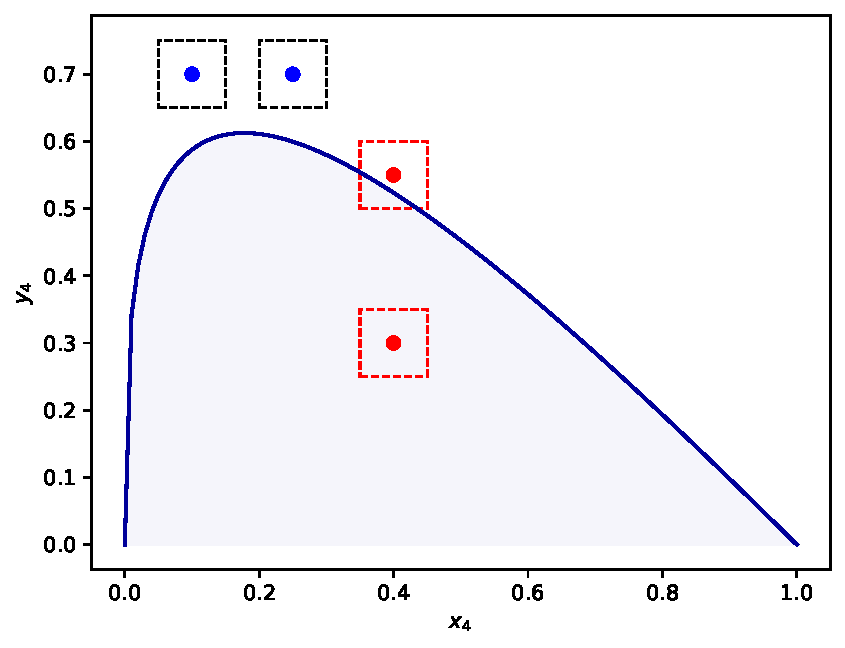
\includegraphics[width = 0.50 \columnwidth]{import/illustrate_lachman_curve.pdf}
  \end{center}
  \caption{
    Illustration of the certification procedure of genuine $4$-PQnG states for the simulated statistical ensembles. The blue line represents the threshold curve $F_{4} (x)$. States with $y_{4} > F_{4}(x_{4})$ are genuine $4$-PQnG states. Four example experimental states are depicted in the figure. The bullet points represent their expectation values obtained by simulating the experiment. The dashed boxes represent their uncertainty and would normally span three standard deviations in both axial directions. The pictured boxes are exaggerated in size for legibility of the illustration. States marked with red bullets failed the certification as they lie either under the threshold curve or their respective uncertainty boxes intersect the curve. States marked with blue bullets are certifiably genuine $4$-PQnG states according to the criteria; their boxes are well above the curve and do not intersect the curve.
  }
  \label{f-otm-il}
\end{figure}

The preparation circuit is evaluated for different amounts of loss in both modes, determined by the transmittances~$\zeta_{1}$ and~$\zeta_{2}$, with varying initial squeezing rates~$r$, and distinct target states~${m}$. Detection events in the simulated experiment are drawn as random samples from a multinomial distribution bootstrapped with the diagonal elements~$\braket{k|\hatrho_{(m)}|k}$ (where ${0 \leq k < 20}$) of the computed density matrix~\eqref{e-pnr-rho}. 

The number of random samples reflects the probability of successful preparation $P_{(m)}$. The probability~\eqref{e-pnr-pro} depends on the initial squeezing rate and the loss in the heralding mode. Given a budget of~$10^{8}$ repetitions available in a single realistic experimental run, only~${\lfloor 10^{8} \times P_{(m)} \rfloor}$ samples are drawn from the distribution and used to estimate the experimental probability distribution~${\overline{p}_{k} \approx \braket{k|\hatrho_{(m)}|k}}$. This random sampling process is repeated~$1000$ times to obtain an ensemble of independent experimental runs for the subsequent statistical analysis.

Certification of the simulated states is achieved with the hierarchical criteria~\cite{lachman2019}. The estimated experimental probabilities~$\overline{p}_{k}$, obtained in each simulated run of the experiment, are used to compute the aggregate random variables characterizing the experimental state,
%
\begin{equation}
  x_{m} = 1 - \sum_{k = 0}^{m} \overline{p}_{k} 
  \quad\text{and}\quad
  y_{m} = \overline{p}_{m} 
  \Qd
\end{equation}
%
Their expectation values and standard deviations, obtained from the ensemble of independent experimental runs, are then used to certify the quantum state resulting from the simulation with the particular choice of~${(m, \zeta_{1}, \zeta_{2}, r)}$ parameters. The experimental state is considered to be a certifiably genuine~$m$-PQnG state if the expectation values lie at least three standard deviations away from the threshold function~$F_{m} (x)$ in both axial directions.

The operating principle of the certification procedure is illustrated in~\figref{f-otm-il} with several example states shown, both passing and failing the certification, along with the actual threshold curve for genuine~$4$-PQnG states.

The extension of this methodology to include CAP detectors is mostly trivial, however, the infinite series in~\eqref{e-cap-pro} and~\eqref{e-cap-rho-kk} stemming from the expression~\eqref{e-cap} must be truncated accordingly. The number of elements considered in the series depends on the particular choice of the~$m$ and~$n$ parameters as these affect how the weight function~${w(i, m, n)}$ behaves. With~$m$ and~$n$ finite and close to each other, the weight function is generally heavy tailed in~$i$ and a sufficiently large cutoff for the summation has to be chosen.

% Results
%
%

\FloatBarrier
\section{Discussion of results}

The main result of this work lies in finding out the maximal tolerable overall loss in the optical experiment for reliable production of certifiable genuine $4$-PQnG states. The use of the hierarchical criteria~\cite{lachman2019} is a necessity due to the realistic loss in preparation of the two mode squeezed states used in the experiment, in their propagation, and low detection efficiency of contemporary detectors with photon number resolving capacity, amplified by the practical unavailability of true PNR detectors. These issues affect the prepared states negatively, manifesting in suboptimal fidelities with the desired state, and leading to poor interpretability of the results. Fidelity alone can not be reliably used to determine whether the prepared state is merely attenuated state of four photons on something else entirely. Unlike fidelity, the hierarchical criteria, based on the stellar rank of the resulting state, offer concrete and unequivocal evidence of non-Gaussian behavior with a greater degree of robustness against loss~\cite{lachman2019}.

\begin{figure}[h]
  \begin{center}
    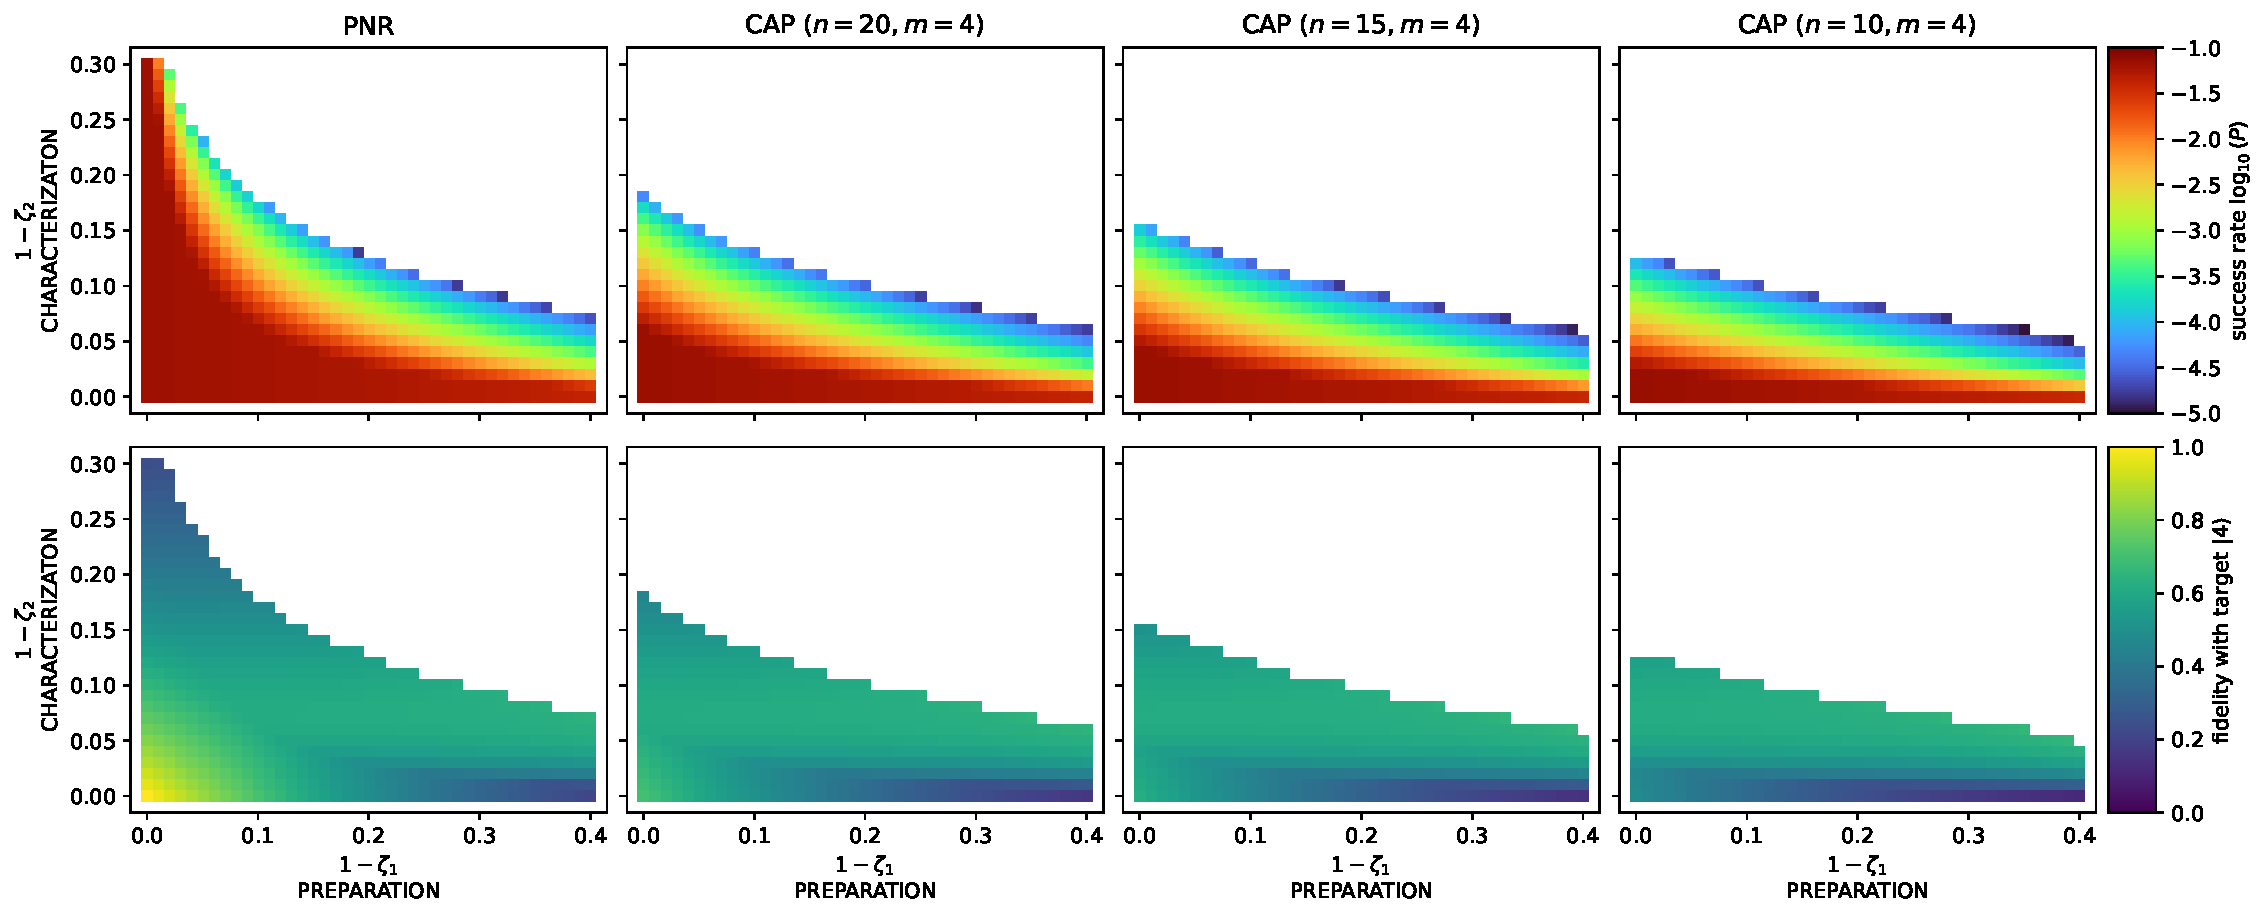
\includegraphics[width = \columnwidth]{import/202411/paper_unified_04.pdf}
  \end{center}
  \caption{
    The tolerable loss in preparation of certifiable genuine $4$-PQnG states. Individual tiles represent the best attainable probability of success (upper row) and the respective fidelity with the state of four photons (lower row). Values in each tile are obtained by optimizing over the initial squeezing rate ${r \leq 10\dB}$. Different heralding detectors are used. The results obtained for a true PNR detector are presented in the leftmost column, while the remaining columns represent CAP detector with ${n = 20, 15, 10}$ constituent avalanche detectors.
  }
  \label{f-res-4}
\end{figure}

% Work from now on.
%

The \figref{f-res-4} showcases the attempts at creating a $4$-PQnG state. The columns represent different modes of detection used in heralding, including true PNR detectors and a range of their approximations using CAP detectors using 20, 15 and 10 individual avalanche photodiodes in a cascade. The upper row presents the best probability of successful preparation, obtained by maximizing over the initial squeezing rate, such that the resulting state is certifiable. The corresponding fidelity with the target state is shown in the lower row. It can be seen that the fidelity is not even close to one, except for the rare case of lossless characterization and heralding using a true PNR detector. All the other modes of detection and lossy cases exhibit fidelities that offer little to no value in terms of qualitative interpretation. The tiles in the plots follow a discrete grid of transmittances. The missing tiles (white space) represent situations where the average number of detection events in single run falls below 1000, that is, given the constraints and assumptions of the simulation, where the probability of success is lower than 10 ppm.

In particular, the \figref{f-otm-4} reveals that it might just be feasible, if the experimentalists get their heads out of their arses and measure the shit out of the states. Of course, it might be advisable that they reduce their loss and dark counts by dipping their detectors in unobtainium and drowning them in liquid helium. He. He. He.


% In each dataset related to the tuple $(m, \zeta_{1}, \zeta_{2})$ of parameters the maximal probability of success is found with respect to the squeezing rate ${r \leq 10\,\dB}$. Both the maximal probability $P_{m}^{\star}$ and the respective optimal squeezing rate ${r^{\star}}$ are visualised in a grid as functions of ${(1 - \zeta_{1}, 1 - \zeta_{2})}$ for each target state $m$. In addition, to present only statistically significant results in the visualisation, grid cells where the probability of success lies below a reasonable threshold set to $10^{-5}$, which guarantees at least $1000$ successful realizations of the state within each experimental run, were blanked out.

% The achievable success rate in preparation and subsequent certification of genuine $m$-photon states is presented in~\figref{f-otm-234}. Each column pertains to the particular target state $m = 2, 3, 4$. The maximal probabilities of success $P_{m}^{\star} (1 - \zeta_{1}, 1 - \zeta_{2})$ are presented in the top row, whereas the corresponding optimal squeezing rates $r^{\star} (1 - \zeta_{1}, 1 - \zeta_{2})$ are provided in the bottom row.
% To reflect on the experimental limitations, the optimization is constrained to squeezing rates limited by $10\,\dB$. The figure also effectively shows the amount of loss that can be tolerated in the experiment.

% In the case of the $2$-photonic state the tolerable loss exceeds $40\%$ in both modes. The probability of success ranges from roughly $10\%$ to $0.1\%$. The higher the loss, the lower the optimal squeezing rate. The tolerable loss is much lower for the state with $3$ photons. The maximal probabilities of success are also reduced. If the state suffers $40\%$ loss during preparation, it can only tolerate at most $20\%$ loss in its characterization. Higher loss leads to success rates lower than the $10^{-5}$ threshold  set earlier; the information obtained in the blanked out region is assumed to be unreliable. Finally, the conditions for the 4 photon state are even less favorable; while it is still possible to tolerate up to $40\%$ loss during preparation, the limit on $1 - \zeta_{2}$ is much more stringent, only about $10\%$ loss is permitted.

% The two mode squeezed vacuum state is assumed to be ideal. The photon number resolving detectors are also presumed to be perfect with unit quantum efficiency. In realistic experiments these assumptions are never true, however, both the inefficiencies in detection and preparation of the squeezed state can be modeled with loss. Consequently the presented results cover these imperfect cases as well since any loss in the initial squeezed state generation are subsumed in the detection losses.


\begin{figure}[h]
  \begin{center}
    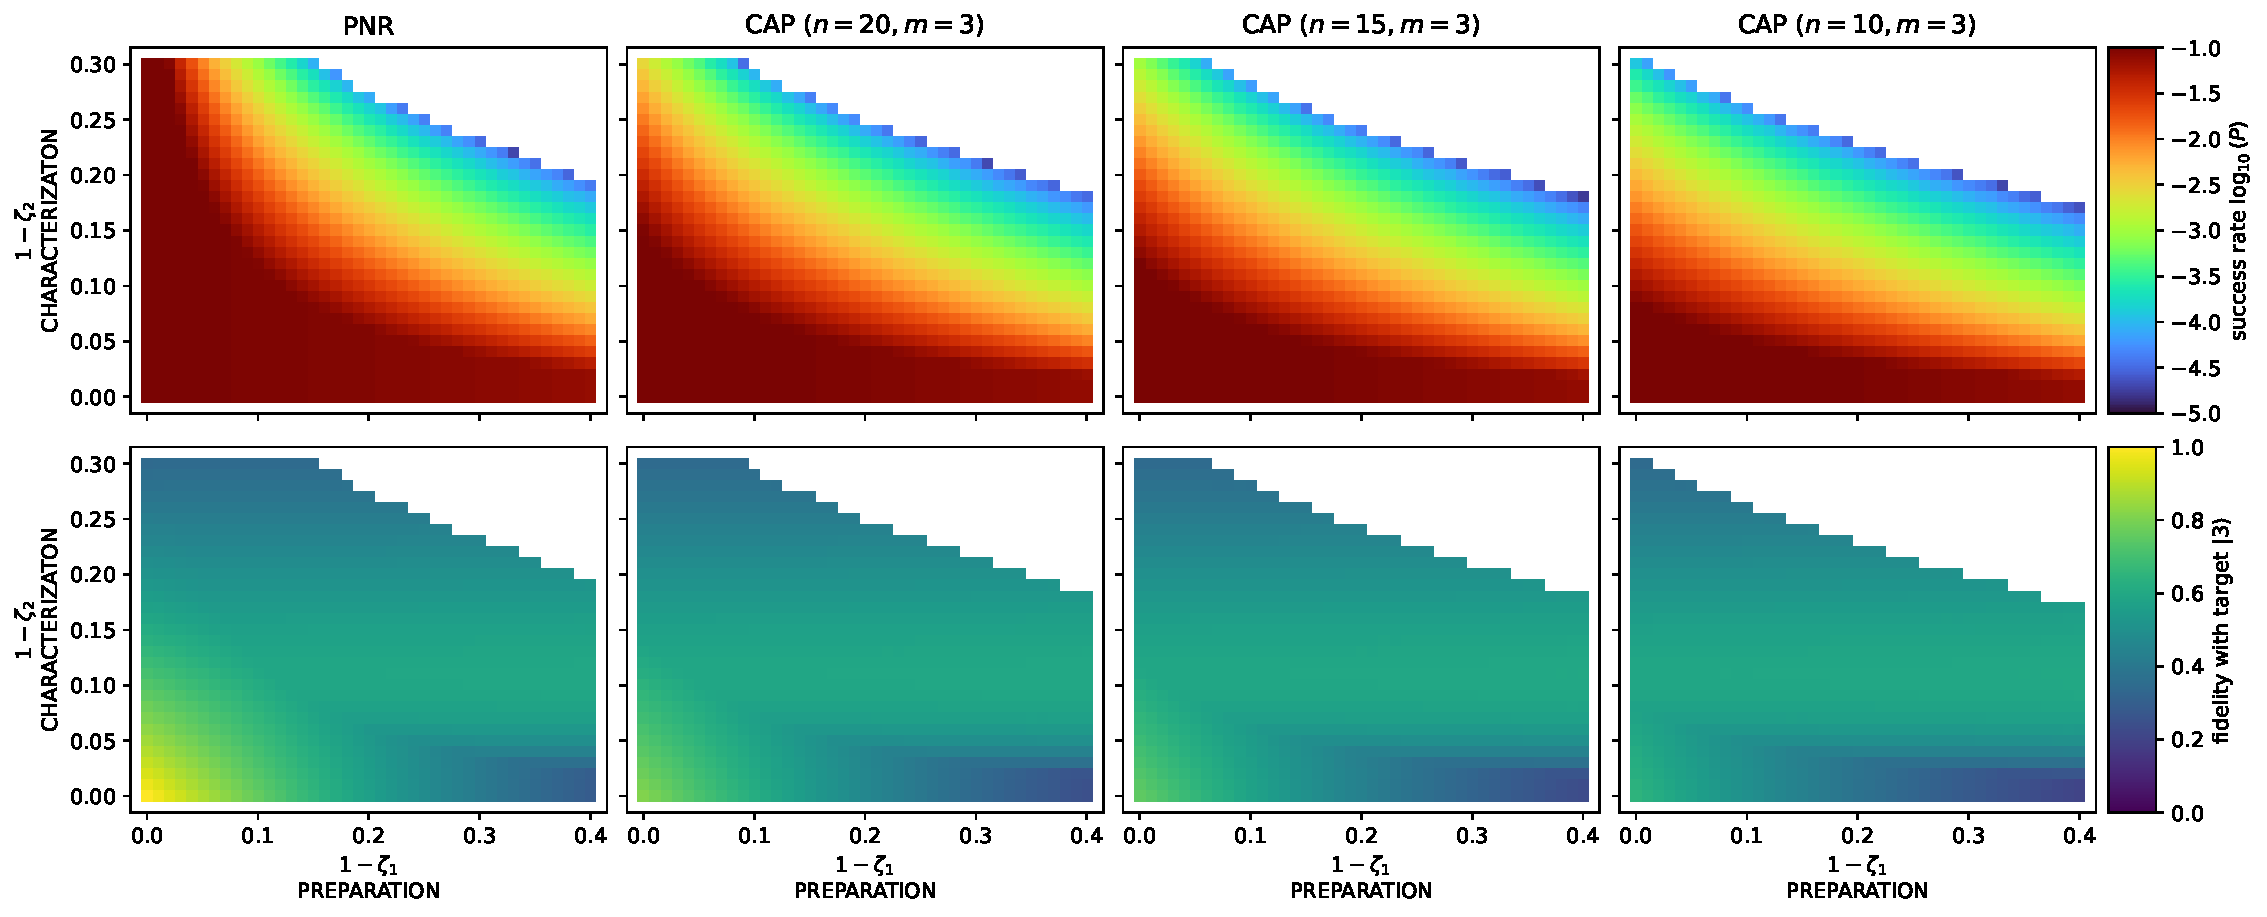
\includegraphics[width = \columnwidth]{import/202411/paper_unified_03.pdf}
  \end{center}
  \caption{
    % The tolerable loss in preparation and subsequent certification of genuine $m$-photon states. Results for target states $m = 2, 3, 4$ are shown in columns. The maximal probabilities $P_{m}^{\star}$ of successful preparation of the certifiable target state, given the particular combination of loss $1 - \zeta_{1}$ incurred during preparation and the loss $1 - \zeta_{2}$ affecting the certification, are presented using a logarithmic scale in the top row. The optimization is constrained to squeezing rates limited by $10\,\dB$. The respective optimal squeezing rates $r^{\star}$ are provided in the bottom row.
  }
  \label{f-otm-3}
\end{figure}

\begin{figure}[h]
  \begin{center}
    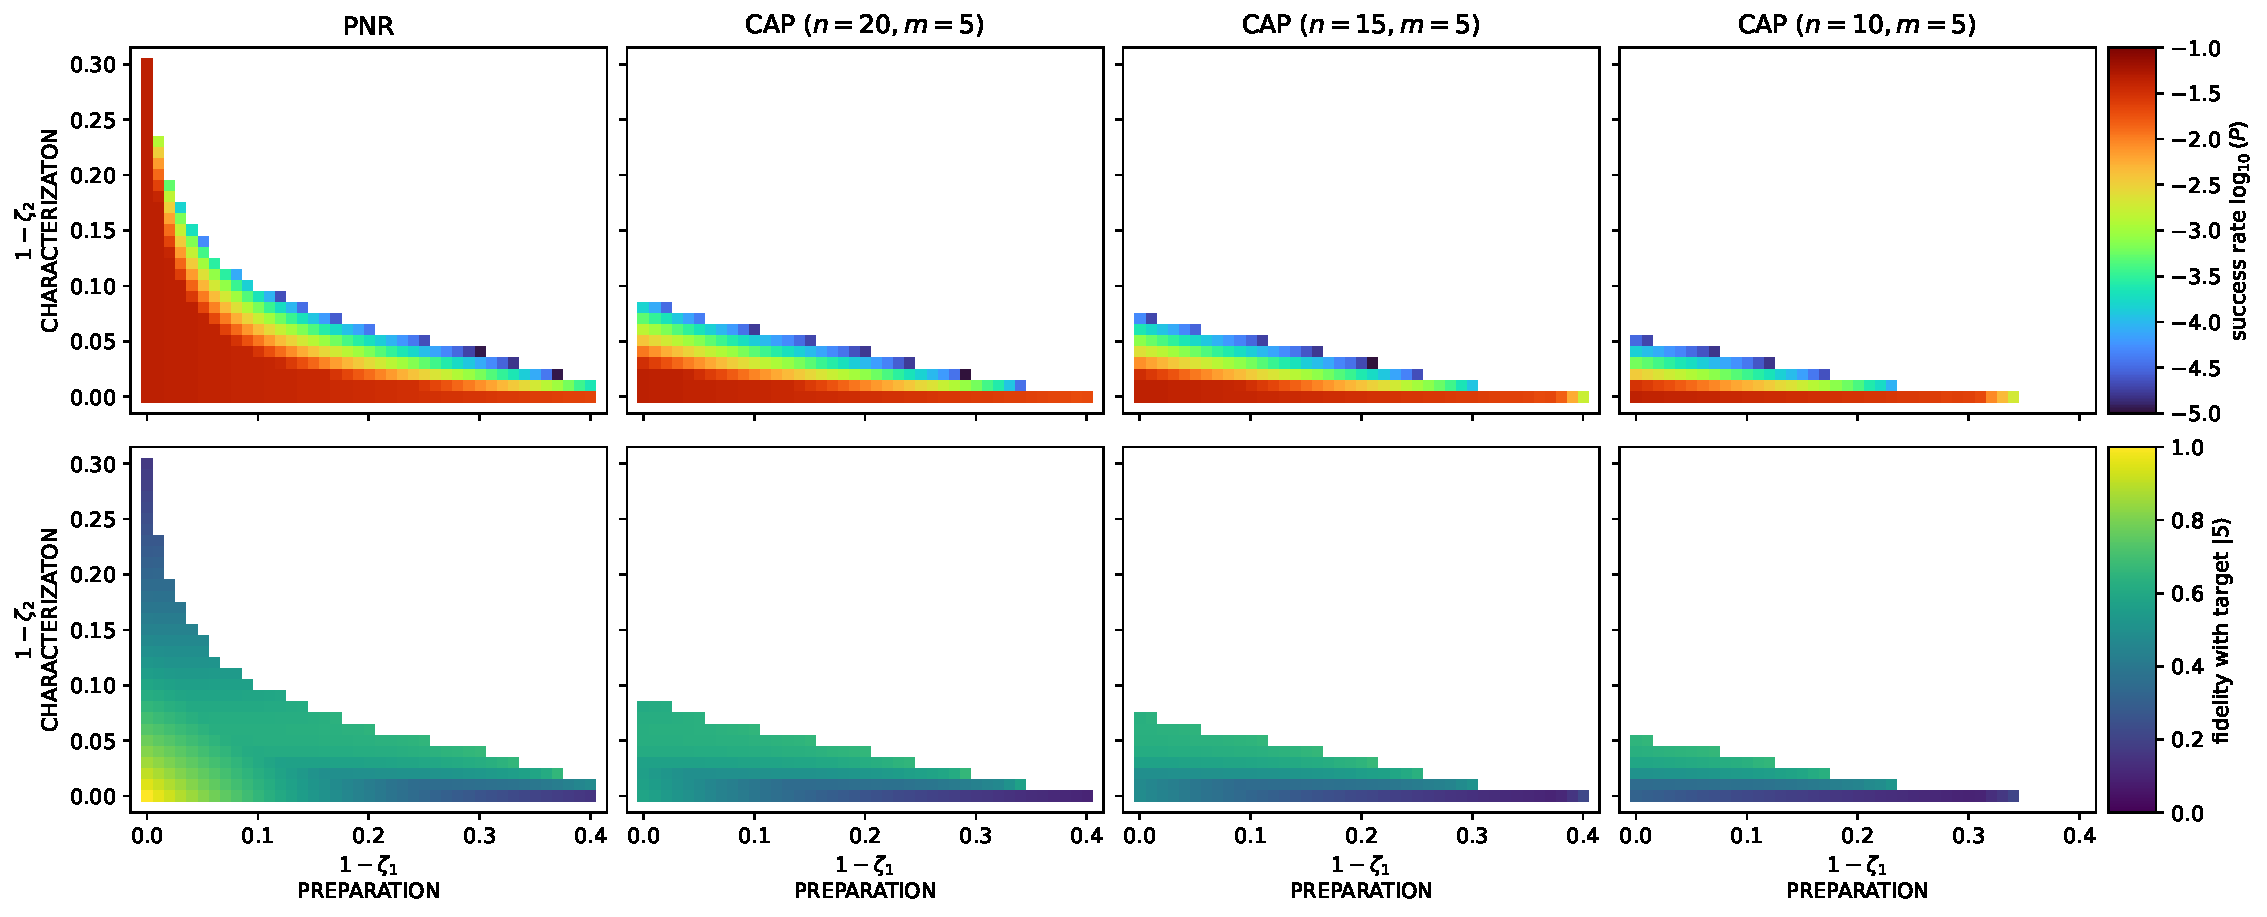
\includegraphics[width = \columnwidth]{import/202411/paper_unified_05.pdf}
  \end{center}
  \caption{
    % The tolerable loss in preparation and subsequent certification of genuine $m$-photon states. Results for target states $m = 2, 3, 4$ are shown in columns. The maximal probabilities $P_{m}^{\star}$ of successful preparation of the certifiable target state, given the particular combination of loss $1 - \zeta_{1}$ incurred during preparation and the loss $1 - \zeta_{2}$ affecting the certification, are presented using a logarithmic scale in the top row. The optimization is constrained to squeezing rates limited by $10\,\dB$. The respective optimal squeezing rates $r^{\star}$ are provided in the bottom row.
  }
  \label{f-otm-5}
\end{figure}

% Conclusions
%
%

\FloatBarrier
\section{Conclusions}

The results presented in this chapter offer an insight into feasible experimental preparation of certifiable genuine $m$-photon states for $m = 2, 3, 4$. While preparation of quantum states of travelling light of up to three photons has already seen its experimental realization~\cite{yukawa2013a}, the construction of a $4$-photon state of travelling light still remains an open problem that will perhaps benefit from the analysis.

% References
%
% 

\FloatBarrier
\printbibliography[heading = bibnumbered]

\end{document}

% vim: linebreak breakindent breakindentopt=shift\:-2 showbreak=↳\  syntax=tex colorcolumn=
